% -*- coding: utf-8 -*-
\documentclass[12pt]{article}
\usepackage{amssymb}%为了打印出反斜杠
\usepackage{listings}
\usepackage{ctex}
\usepackage{graphicx}
\usepackage[a4paper, body={18cm,22cm}]{geometry}
\usepackage{amsmath,amssymb,amstext,wasysym,enumerate,graphicx}
\usepackage{float,abstract,booktabs,indentfirst,amsmath}
\usepackage{array}
\usepackage{booktabs} %调整表格线与上下内容的间隔
\usepackage{multirow}
\usepackage{diagbox}
\usepackage{color}%字体颜色包
\usepackage[colorlinks,linkcolor=blue,urlcolor=black,anchorcolor=blue,citecolor=blue,]{hyperref}%超链接包
\renewcommand\arraystretch{1.4}
\usepackage{indentfirst}
\setlength{\parindent}{2em}

\geometry{left=2.8cm,right=2.2cm,top=2.5cm,bottom=2.5cm}
%\geometry{left=3.18cm,right=3.18cm,top=2.54cm,bottom=2.54cm}

\graphicspath{{figures/}}

\title{\heiti 作业五.Wapiti序列标注的CRF实现和.pat模板测试}

\begin{document}

	\maketitle
	
	\vspace{5cm}
	
	\begin{table}[h]
		\centering
		\begin{Large}
			\begin{tabular}{p{3cm} p{7cm}<{\centering}}
				学  \qquad  校: &  华中农业大学     \\ \cline{2-2}
				学院班级:      & 信息学院生信1801班   \\ \cline{2-2}
				姓  \qquad  名: & 邓启东 \\ \cline{2-2}
				学  \qquad  号: & 2018317220103 \\ \cline{2-2}
				指导教师:       &夏静波 \\ \cline{2-2}
			\end{tabular}
		\end{Large}		
	\end{table}
	
	\newpage%一个新的页面

	\tableofcontents
	
	\newpage
	\section{实验目的}

	\section{实验材料与方法}
\subsection{CRF算法介绍}
条件随机域模型是由Lafferty在2001年提出的一种典型的判别式模型。它在观测序列的基础上对目标序列进行建模,重点解决序列化标注的问题。条件随机域模型既具有判别式模型的优点,又具有产生式模型考虑到上下文标记间的转移概率,以序列化形式进行全局参数优化和解码的特点,解决了其他判别式模型(如最大熵马尔科夫模型)难以避免的标记偏置问题。
\subsection{wapiti工作环境配置}
wapiti是一个实现CRF算法的工具 安装好就编译成为了二进制文件
解压整个项目压缩文件,并解压其中的AGAC语料库,其中有训练集和测试集。使用unrar解压失败(见图\ref{mmm})。\par
\begin{figure}[H]
  \centering
  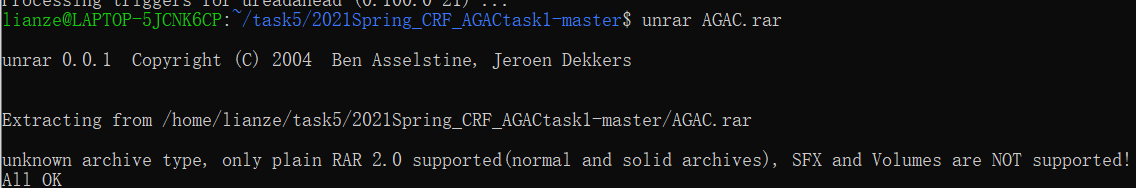
\includegraphics[scale=0.5]{./picture/unrar.png} %1.png是图片文件的相对路径
  \caption{未知类型:unrar无法解压} %caption是图片的标题
  \label{mmm} %此处的label相当于一个图片的专属标志,目的是方便上下文的引用
\end{figure}
改换7zip,使用代码sudo apt-get install p7zip-full p7zip-rar安装,代码7z x AGAC.rar解压。解压成功。\par
\subsection{数据描述}
实际上,原本的AGAC语料库文件我们在任务一中是见到过的,原本是一个jason格式的文件。jason文件是以字典的形式储存text和denotations的。经过Python的nltk包处理之后,将实体标签和分词根据根据未知信息对应,就得到了相应形式的BIO文件,作为我们的训练集。\par
我们随便打开一篇,例如打开/AGAC/test\_split/ddd\_split\_211.txt这一篇。第一列便是我们的input,其实就是序列标注的句子,每一行就是句子的一个单词。而它的实际标签就是最后一列,以BIO的形式呈现,例如B-Var、B-Gene、B-Enzyme、I-MPA等等。以这种方式就可以很好的对多个单词组成的短语进行标注(见图\ref{xxxww})。\par
这里明显看到Denys-Drash syndrome这个疾病的边界被很好的标注出来了。\par
\begin{figure}[H]
  \centering
  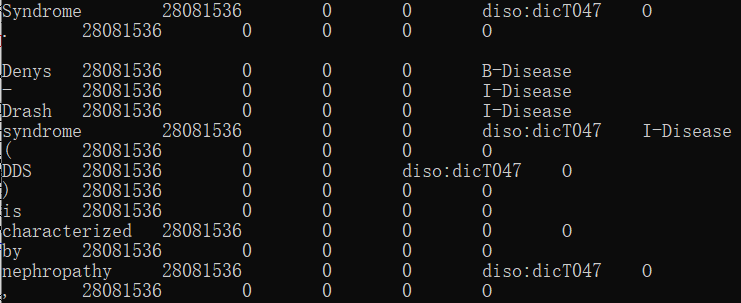
\includegraphics[scale=0.6]{./picture/form.png} %1.png是图片文件的相对路径
  \caption{标注格式} %caption是图片的标题
  \label{xxxww} %此处的label相当于一个图片的专属标志,目的是方便上下文的引用
\end{figure}

这里的训练集包含500篇摘要,由标注员手工标注的。由语料库开发到黄金数据库花费了20个月。但是也意味着这个训练集非常的准确。\par
第一列语料库文件中的内容分割后得到的,包括单词,数字和标点符号\par
第二列的数字是PMID\par
第五列的diso是自己造的词典,收纳了和不良反应的词,表示diso中的副作用,这个词典在diso-DISO.dic文件可以看到。\par
而测试集的标签全部为O。
\subsection{训练模型}
wapiti train -a sgd-l1 -t 3 -i 10 -p pat/Tok321dis.pat <(cat AGAC/train\_split/*.txt) AGAC/mod/AGAC\_train.mod \par
这句代码其实就是把AGAC/train\_split/路径下所有的语料库文件数据用于训练。\par
“<”是指将这个训练集进去。\par
-p 指定模板文件,只有wapiti这么提,其实是特征函数的生成方式,Tok321dis.pat中就是特征函数。\par
我们打开这个文件,见图\ref{fffff}。

\begin{figure}[H]
  \centering
  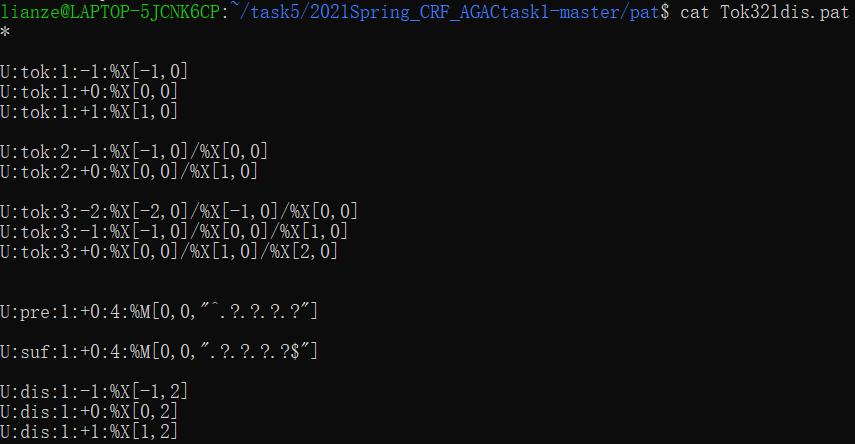
\includegraphics[scale=0.5]{./picture/feature.png} %1.png是图片文件的相对路径
  \caption{特征函数生成模板} %caption是图片的标题
  \label{fffff} %此处的label相当于一个图片的专属标志,目的是方便上下文的引用
\end{figure}
训练出来的模型便保存在了AGAC\_train.mod中。
由于开头第一个字母是U,这样相对于输出序列而言的表示方式是Unigram模板,意思是前一个数据,后一个数据和当前的数据构成的上下文对当前标签的影响,还有一种表示方式是Bigram模板,这个模板会考虑当前输出标签和上一个输出标签。\par
模板文件中的每一行代表一个template。每一个template中,专门的宏\%x[row,col]用于确定输入数据中的一个token。row用于确定与当前的token的相对行数。col用于确定列。\par
结果如下图所示(见图\ref{221aa})。
\begin{figure}[H]
  \centering
  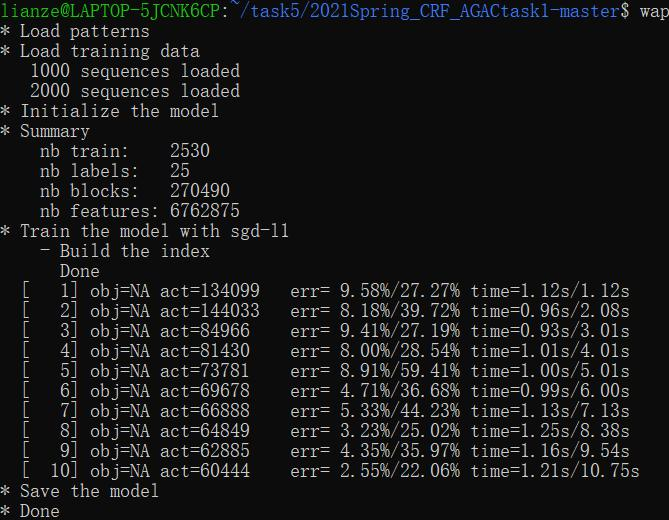
\includegraphics[scale=0.6]{./picture/pretrain.png} %1.png是图片文件的相对路径
  \caption{pretrain} %caption是图片的标题
  \label{221aa} %此处的label相当于一个图片的专属标志,目的是方便上下文的引用c
\end{figure}
可以看到由特征模板学到的特征有6,762,875。
\subsection{预测标签}
wapiti label -c -m AGAC/mod/AGAC\_train.mod <(cat AGAC/test\_split/*.txt) AGAC/train\_out.tab\par
也就是拿训练好的模型来预测test\_split目录下的那250篇文献,如下图,可以看到每一个标签的预测情况(见图\ref{sad})。
如果打开train\_out.tab,可以直接看到第五列后面多了一列预测。可以和实际的结果相互比较。
\begin{figure}[H]
  \centering
  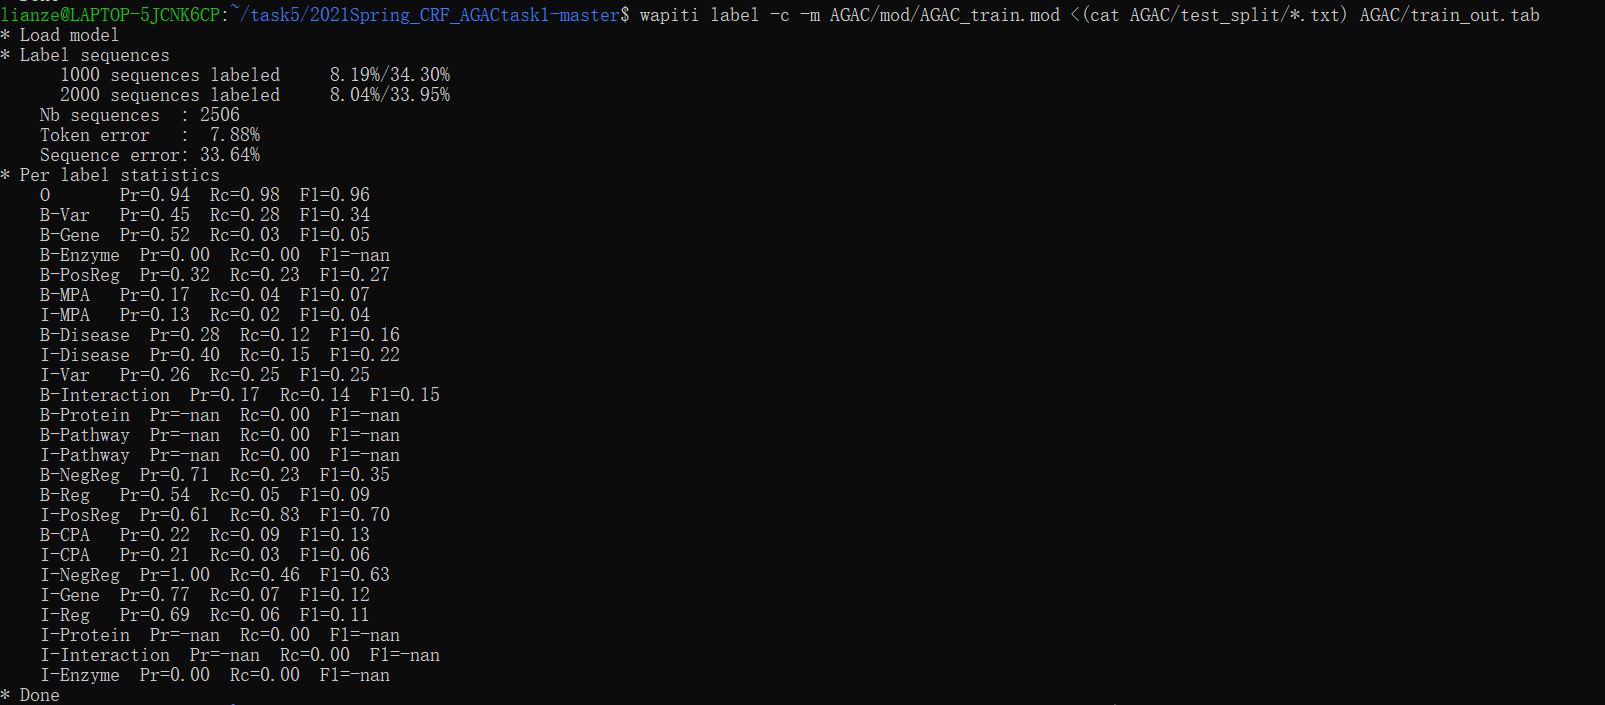
\includegraphics[scale=0.4]{./picture/predict.png} %1.png是图片文件的相对路径
  \caption{标签预测完成} %caption是图片的标题
  \label{sad} %此处的label相当于一个图片的专属标志,目的是方便上下文的引用
\end{figure}
O本身就占有大部分,所以准确度和召回率都很高自不必说。
\subsection{评估结果}
perl conlleval.pl -d \$'$\setminus$ t'<AGAC/train\_out.tab | tee AGAC/train\_out.eval \par
评估结果见下图(图/ref{result})
\begin{figure}[H]
  \centering
  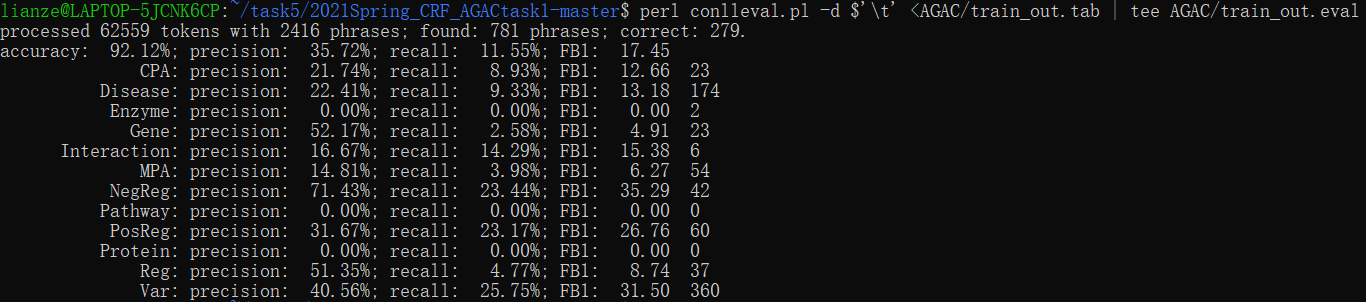
\includegraphics[scale=0.4]{./picture/result.png} %1.png是图片文件的相对路径 
  \caption{预测结果评估} %caption是图片的标题
  \label{result} %此处的label相当于一个图片的专属标志,目的是方便上下文的引用
\end{figure}



\section{.pat模板修改测试}
\subsection{.pat模板修改}
为了提高结果的FB1的值,则需要修改.pat文件里面的特征模板,特征的生成方式变得更加复杂,tok可以提高到4。\par
修改后的.pat文件如下图所示(见下图\ref{asaddd}):
\begin{figure}[H]
  \centering
  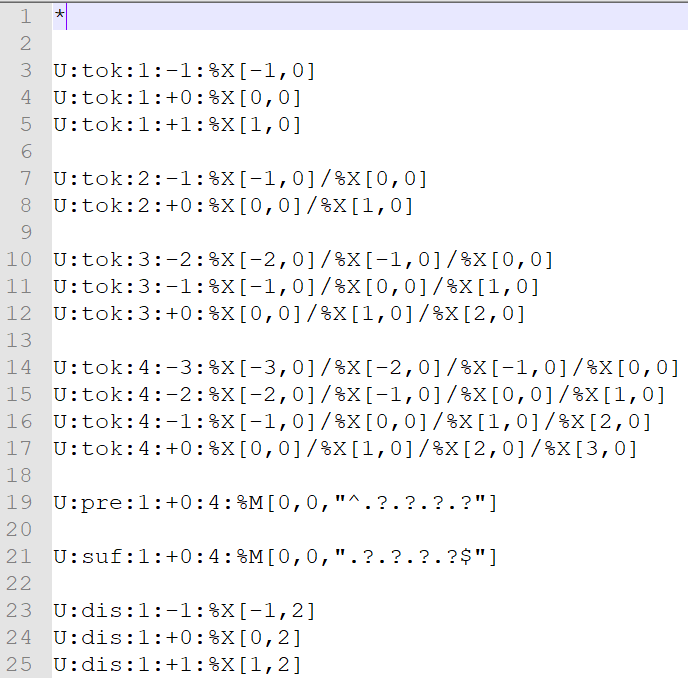
\includegraphics[scale=0.5]{./picture/patchange.png} %1.png是图片文件的相对路径
  \caption{修改后的pat文件} %caption是图片的标题
  \label{asaddd} %此处的label相当于一个图片的专属标志,目的是方便上下文的引用
\end{figure}
\subsection{修改后结果}
这个时候我们的特征已经有12,922,075个了。但是可能是由于特征太多的原因,导致了学习的效果不增反降(见下图\ref{sadasaa})。
\begin{figure}[H]
  \centering
  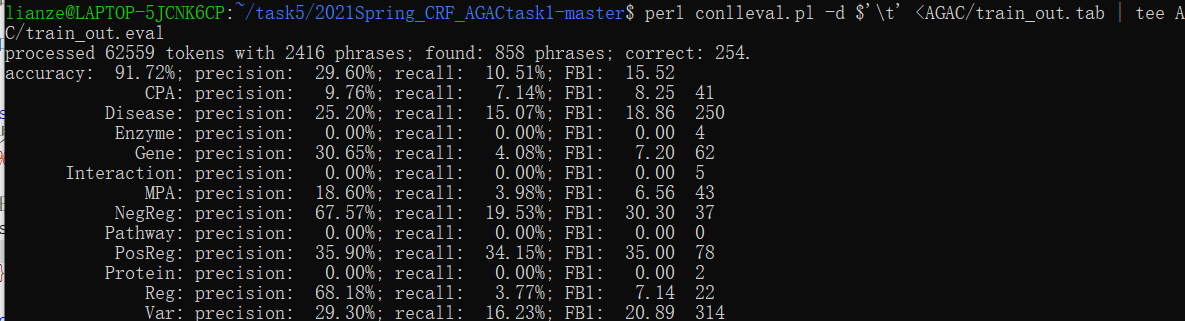
\includegraphics[scale=0.5]{./picture/result2.png} %1.png是图片文件的相对路径
  \caption{预测结果评估} %caption是图片的标题
  \label{sadasaa} %此处的label相当于一个图片的专属标志,目的是方便上下文的引用
\end{figure}
分析原因,估计是语料库还不够大,特征过多导致预测效果不佳。
不过我们此刻还没有放弃,因为FB1的值不增反降。因此我打算插入tok5,查看结果。如果按照理论而言,如果将模板扩增到tok4,那么特征的数量就会多更多更多。如果效果更差,也许特征太多的原因。如果tok5的FB1的值最大,那么说明tok4效果不佳,具体原因不太明白。\par
\subsection{增加到tok5}
我们把U模板扩增到tok5(见下图\ref{256556})。
\begin{figure}[H]
  \centering
  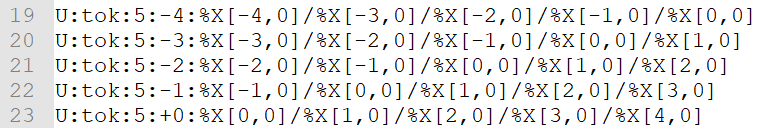
\includegraphics[scale=0.5]{./picture/tok5wa.png} %1.png是图片文件的相对路径
  \caption{增加到tok5} %caption是图片的标题
  \label{256556} %此处的label相当于一个图片的专属标志,目的是方便上下文的引用
\end{figure}
可以明显感受到整个训练、预测、评估的过程所花费的时间长了很多。结果如下图所示(\ref{2123345555})。
\begin{figure}[H]
  \centering
  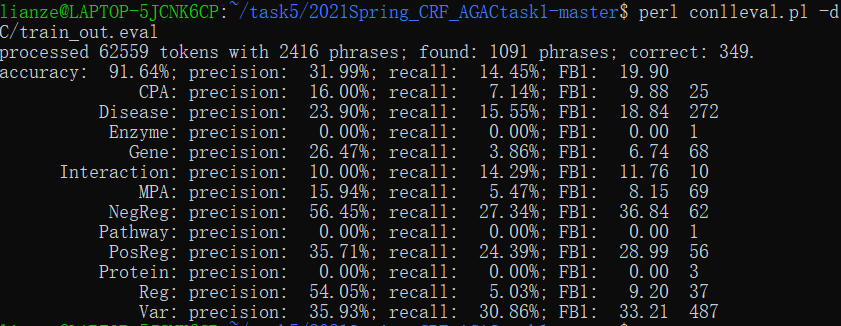
\includegraphics[scale=0.5]{./picture/tok5.png} %1.png是图片文件的相对路径
  \caption{增加到tok5} %caption是图片的标题
  \label{2123345555} %此处的label相当于一个图片的专属标志,目的是方便上下文的引用
\end{figure}
这次看到,FB1的值有明显提高,比tok3整体要好很多。不过部分预测能力也不如tok3,比如对于CPA的识别,tok3的FB1值是12.66而tok5仅有9.88。Interaction这一栏,tok3的FB1值是15.38,tok5是11.76.不过这些都比tok4的Interaction准确率,召回率,FB1均为0要好。\par
这说明tok4本身学到的特征还是有些许问题的。也说明虽然在个别标签反有不足,总体来说增加模板的上下文词数来增加特征函数还是一定程度上可以改进标签预测的效果的。
\section{参考链接}
\begin{enumerate}
\item \href{https://github.com/bionlp-hzau/2021Spring_CRF_AGACtask1}{\underline{原项目Github链接}}
\item \href{https://blog.csdn.net/m0_51732188/article/details/109318840}{\underline{参考博客}}

\end{enumerate}


\bibliographystyle{unsrt}
\bibliography{MyCitation}% Produces the bibliography via BibTeX.
\end{document}


















%%%%%%%%%%%%%%%%%%%%%%%%%%%%Library%%%%%%%%%%%%%%%%%%%%%%%%%%%%%%%%%%%%%%%

% 1. 脚注用法
	LaTeX\footnote{Latex is Latex} is a good software

%2. 强调
	\emph{center of percussion} %[Brody 1986], %\lipsum[5]

%3. 随便生成一段话
	\lipsum[4]

%4. 列条目
	\begin{itemize}
	\item the angular velocity of the bat,
	\item the velocity of the ball, and
	\item the position of impact along the bat.
	\end{itemize}

%5. 表格用法
	\begin{table}[h]
	\centering  
	\begin{tabular}{c|cc}
		\hline
		年份 & \multicolumn{2}{c}{指标}\\
		\hline
		2017 & 0.9997 & 0.0555 \\
		2018 & 0.9994 & 0      \\
		2019 & 0.9993 & 0      \\
		\hline
	\end{tabular}
	\caption{NAME}\label{SIGN}
	\end{table}

	\begin{center}
		\begin{tabular}{c|cclcrcc}
			\hline
			Year & theta & $S_1^-$ & $S_2^-$ & $S_3^-$ & $S_4^+$ & $S_5^+$ & $S_6^+$ \\%表格标题
			\hline
			2016 & 1      & 0      & 0 & 0.0001 & 0      & 0      & 0 \\
			2017 & 0.9997 & 0.0555 & 0 & 0.2889 & 0.1844 & 0.463  & 0 \\
			2018 & 0.9994 & 0      & 0 & 0.0012 & 0.3269 & 0.7154 & 0 \\
			2019 & 0.9993 & 0      & 0 & 0      & 0.4325 & 1.0473 & 0 \\
			2020 & 0.9991 & 0      & 0 & 0      & 0.5046 & 1.2022 & 0 \\
			2021 & 0.999  & 0      & 0 & 0      & 0.5466 & 1.2827 & 0 \\
			2022 & 0.9989 & 0.0017 & 0 & 0.3159 & 0.562  & 1.2995 & 0 \\
			2023 & 0.9989 & 0      & 0 & 0.0109 & 0.5533 & 1.2616 & 0 \\
			2024 & 0.9989 & 0      & 0 & 0      & 0.5232 & 1.1769 & 0 \\
			2025 & 0.9989 & 0      & 0 & 0.1009 & 0.4738 & 1.0521 & 0 \\
			2026 & 0.9991 & 0      & 0 & 0      & 0.4071 & 0.8929 & 0 \\
			2027 & 0.9992 & 0.0004 & 0 & 0.1195 & 0.3248 & 0.7042 & 0 \\
			2028 & 0.9994 & 0.0164 & 0 & 0.046  & 0.2287 & 0.4902 & 0 \\
			2029 & 0.9997 & 0      & 0 & 0.0609 & 0.12   & 0.2545 & 0 \\
			2030 & 1      & 0      & 0 & 0      & 0      & 0      & 0 \\
			\hline
		\end{tabular}
	\end{center}

%6. 数学公式
	\begin{equation}
		a^2 = a * a\label{aa}
	\end{equation}
	
	\[
	\begin{pmatrix}{*{20}c}
	{a_{11} } & {a_{12} } & {a_{13} }  \\
	{a_{21} } & {a_{22} } & {a_{23} }  \\
	{a_{31} } & {a_{32} } & {a_{33} }  \\
	\end{pmatrix}
	= \frac{{Opposite}}{{Hypotenuse}}\cos ^{ - 1} \theta \arcsin \theta
	\]
	
	\[
	p_{j}=\begin{cases} 0,&\text{if $j$ is odd}\\
	r!\,(-1)^{j/2},&\text{if $j$ is even}
	\end{cases}
	\]
	
	
	\[
	\arcsin \theta  =
	\mathop{{\int\!\!\!\!\!\int\!\!\!\!\!\int}\mkern-31.2mu
		\bigodot}\limits_\varphi
	{\mathop {\lim }\limits_{x \to \infty } \frac{{n!}}{{r!\left( {n - r}
				\right)!}}} \eqno (1)
	\]

%7. 双图并行
	\begin{figure}[h]
		% 一个2*2图片的排列
		\begin{minipage}[h]{0.5\linewidth}
			\centering
			\includegraphics[width=0.8\textwidth]{./figures/0.jpg}
			\caption{Figure example 2}
		\end{minipage}
		\begin{minipage}[h]{0.5\linewidth}
			\centering
			\includegraphics[width=0.8\textwidth]{./figures/0.jpg}
			\caption{Figure example 3}
		\end{minipage}
	\end{figure}

%8. 单张图片部分
	\begin{figure}[h]
		%\small
		\centering
		\includegraphics[width=12cm]{./figures/mcmthesis-aaa.eps}
		\caption{Figure example 1} \label{fig:aa}
	\end{figure}

%%%%%%%%%%%%%%%%%%%%%%%%%%%%%%%%%%%%%%%%%%%%%%%%%%%%%%%%%%%%%%%%%%%%%%%%%%%%%
\begin{minipage}{0.5\linewidth}
	\begin{tabular}{|c|c|c|}
		\hline
		\multicolumn{2}{|c|}{\multirow{2}{*}{合并}}&测试\\
		\cline{3-3}
		\multicolumn{2}{|c|}{}& 0.9997  \\
		\hline
		2019 & 0.9993 & 0 \\
		\hline
	\end{tabular}
\end{minipage}

\begin{minipage}{0.5\linewidth}
	\begin{tabular}{c|ccc}
		\hline
		年份 & \multicolumn{3}{c}{指标}\\
		\hline
		\multirow{3}{*}{合并}&2017 & 0.9997 & 0.0555 \\
		&2018 & 0.9994 & 0      \\
		&2019 & 0.9993 & 0      \\
		\hline
	\end{tabular}
\end{minipage}



	\begin{table}[h]
	\centering	
	\begin{Large}
		\begin{tabular}{p{4cm} p{8cm} < {\centering}}
			\hline
			院\qquad 系: & 信息工程学院 \\
			\hline
			团队名称: & PlantBook Team \\
			\hline
			分\qquad 组: & 第0组1号 \\
			\hline
			日\qquad 期: & 2017年10月28日 \\
			\hline
			指导教师: & 吱吱吱\\
			\hline
		\end{tabular}
	\end{Large}
\end{table}


\ctexset{
	section={
		format+=\heiti \raggedright,
		name={,、},
		number=\chinese{section},
		beforeskip=1.0ex plus 0.2ex minus .2ex,
		afterskip=1.0ex plus 0.2ex minus .2ex,
		aftername=\hspace{0pt}
	},
}

	\begin{table}[h]
	\centering
	\begin{Large}
		\begin{tabular}{p{3cm} p{7cm}<{\centering}}
			院  \qquad  系: & 信息工程学院           \\ \cline{2-2}
		\end{tabular}
	\end{Large}		
\end{table}
\thispagestyle{empty}
\newpage
\thispagestyle{empty}
\tableofcontents
\thispagestyle{empty}
\newpage
\setcounter{page}{1}

% 9. 代码

\usepackage{listings}
\usepackage{xcolor}
\lstset{
	numbers=left, 
	numberstyle= \tiny, 
	keywordstyle= \color{ blue!70},
	commentstyle= \color{red!50!green!50!blue!50}, 
	frame=shadowbox, % 阴影效果
	rulesepcolor= \color{ red!20!green!20!blue!20} ,
	escapeinside=``, % 英文分号中可写入中文
	xleftmargin=2em,xrightmargin=2em, aboveskip=1em,
	basicstyle=\footnotesize,
	framexleftmargin=2em
}
